\documentclass{article}
\usepackage{url}
\usepackage[tight]{subfigure}
\usepackage{graphicx}
\usepackage{float}
\usepackage{listings}
\author{Sean Flaherty}
\title{Probabilistic Dust Storm Predictive Modeling}
\begin{document}
\maketitle
\section{Introduction}
Dust storms have numerous adverse effects to populated areas, including disruptions to communications and traffic, damage to property and equipment, and respiratory health hazards. These effects are caused by reduced visibility and dust particles suspended in the air. Further effects, such as damage to croplands, are caused by sediment that settles after dust storms. To mitigate the damages caused by dust storms, an early warning system is ncessary. To develop an early warning system, a predictive model is needed. Currently, there exists a numerical model known as the Dust Regional Atmospheric Model, or DREAM. DREAM models dust particle movement such that it can predict a dust event up to 72 hours in advance, and attempt to predict the movement of dust particle systems \cite{unep}. 

The Public Health Applications in Remote Sensing (PHaiRS) project aimed to assimilate higher-resolution data into a version of the DREAM model adapted for the Southwestern United States referred to as DREAM/SW with the goal of increasing the prediction accuracy of DREAM/SW and improving public respiratory health outcomes. While parameters of increased resolution were in agreement for overall dust movement patterns, increasing the resolution of parameter data had a plateau effect in accuracy and public health outcome \cite{phairs}. Because DREAM is a deterministic predictive model, in order to determine what variables may be stronger predictors for future dust events, a probabilistic model is necessary.

\subsection{Research Overview}
A previous study on probabilistic modeling of dust events uses 500mB geopotential height patterns as a univariate predictor of dust events using grayscale image processing. In this study, 500mB geopotential heights are recorded in the southwestern United States and northern Mexico from 2011 to 2014 and dates are classified as dust or non-dust days. To create a more separable data set, days before and after dust days are omitted from the data. The training data for the study is formatted into a grayscale raster image, and the images for dust and non-dust days are averaged together. To perform the classification, a sample raster image is compared to the average dust day image using zero mean normalized cross-correlation (ZNCC). This technique determined that dust storms occurred as a result of a low pressure system in northern New Mexico often called the "Albuquerque low," although it only worked as a predictor of more major dust events, and could not predict smaller or more short-lived events \cite{500mb}.

Due to the limitations of only using 500mB geopotential heighs as a predictor for dust events, a model is needed that not only predicts large-scale dust events from a major low-pressure system, but one that also predicts small and short-lived events. The objective of this project is to create a probabilistic predictive model for dust events that achieves this goal using multiple variables as predictors. Using rapid update cycle (RUC) forecast data from 2011 to 2014, a wider range of variables is available for a predictive modeling. The larger number of variables, however, introduces the curse of dimensionality \cite{tan}. In order to have a meaningful and accurate prediction, the dimensionality must be reduced such that only the strongest predictors of dust events are used. To do so, instead of using the proper training data, a principal component analysis (PCA) of the data is used instead.
\section{Methodology}
\subsection{Data}
The data used for this study is retrieved from the NOAA Operational Model Archive and Distribution System (NOMADS). The particular forecast models used to create a predictive model are the Rapid Refresh (RAP) and Rapid Update Cycle (RUC) models. NOMADS makes its data available via HTTPS or FTP. For this project, the data is downloaded via HTTPS using the GNU Wget utility. For a preliminary model, only data recorded at 18:00 GMT is used. In order to retrieve this data, the following Wget command is invoked:
\begin{verbatim}
wget -r -np -nd -A 'ruc2anl_130_*_1800_000.grb2' -e 
robots=off https://nomads.ncdc.noaa.gov/data/rucanl
\end{verbatim}

This command reads all files from each directory in the RAP/RUC parent directory, and downloads them to a single local folder \cite{wget}. This particular command gathers all .grb2 files with a 13km resolution, although 25.2km resolution is also available. The command also does not retrieve all files, as before 2007 files existed in .grb format.

The .grb and .grb2 formats are two versons of the GRIdded Binary (GRIB) format, which is the World Meteorological Organization's standard for storing observation and forecast data. The file format contains a header that describes the contents of the file, as well as binaries for each recorded weather parameter. The binaries are stored in a raster, with each point in that raster corresponding to the recorded data for a specific latitude and longitude.

In order to read a GRIB file in Python, the pygrib library is used. The library allows the files to be opened as iterators containing gribmessage objects, each of which contains the data for a weather parameter. Each gribmessage contains a parameter name, height and time information, the latitudes and longitudes for which the data is recorded, and the corresponding parameter information for each latitude and longitude \cite{pgdoc}. Because this project is concerned with predicting dust storms on a local scale, a single index is taken from the 2-dimensional data array for each parameter.

Data is visualized using the NOAA Weather and Climate Tool. Using this program, GRIB files can be opened and and weather maps of any desired parameter can be displayed. In figure ~\ref{fig:map}, a map is generated using the WCT viewer to visualize 500mB geopotential height during a large-scale dust event. This particular event shows the "Albuquerque Low" pressure system.

\begin{figure}[H]
	\label{fig:map}
	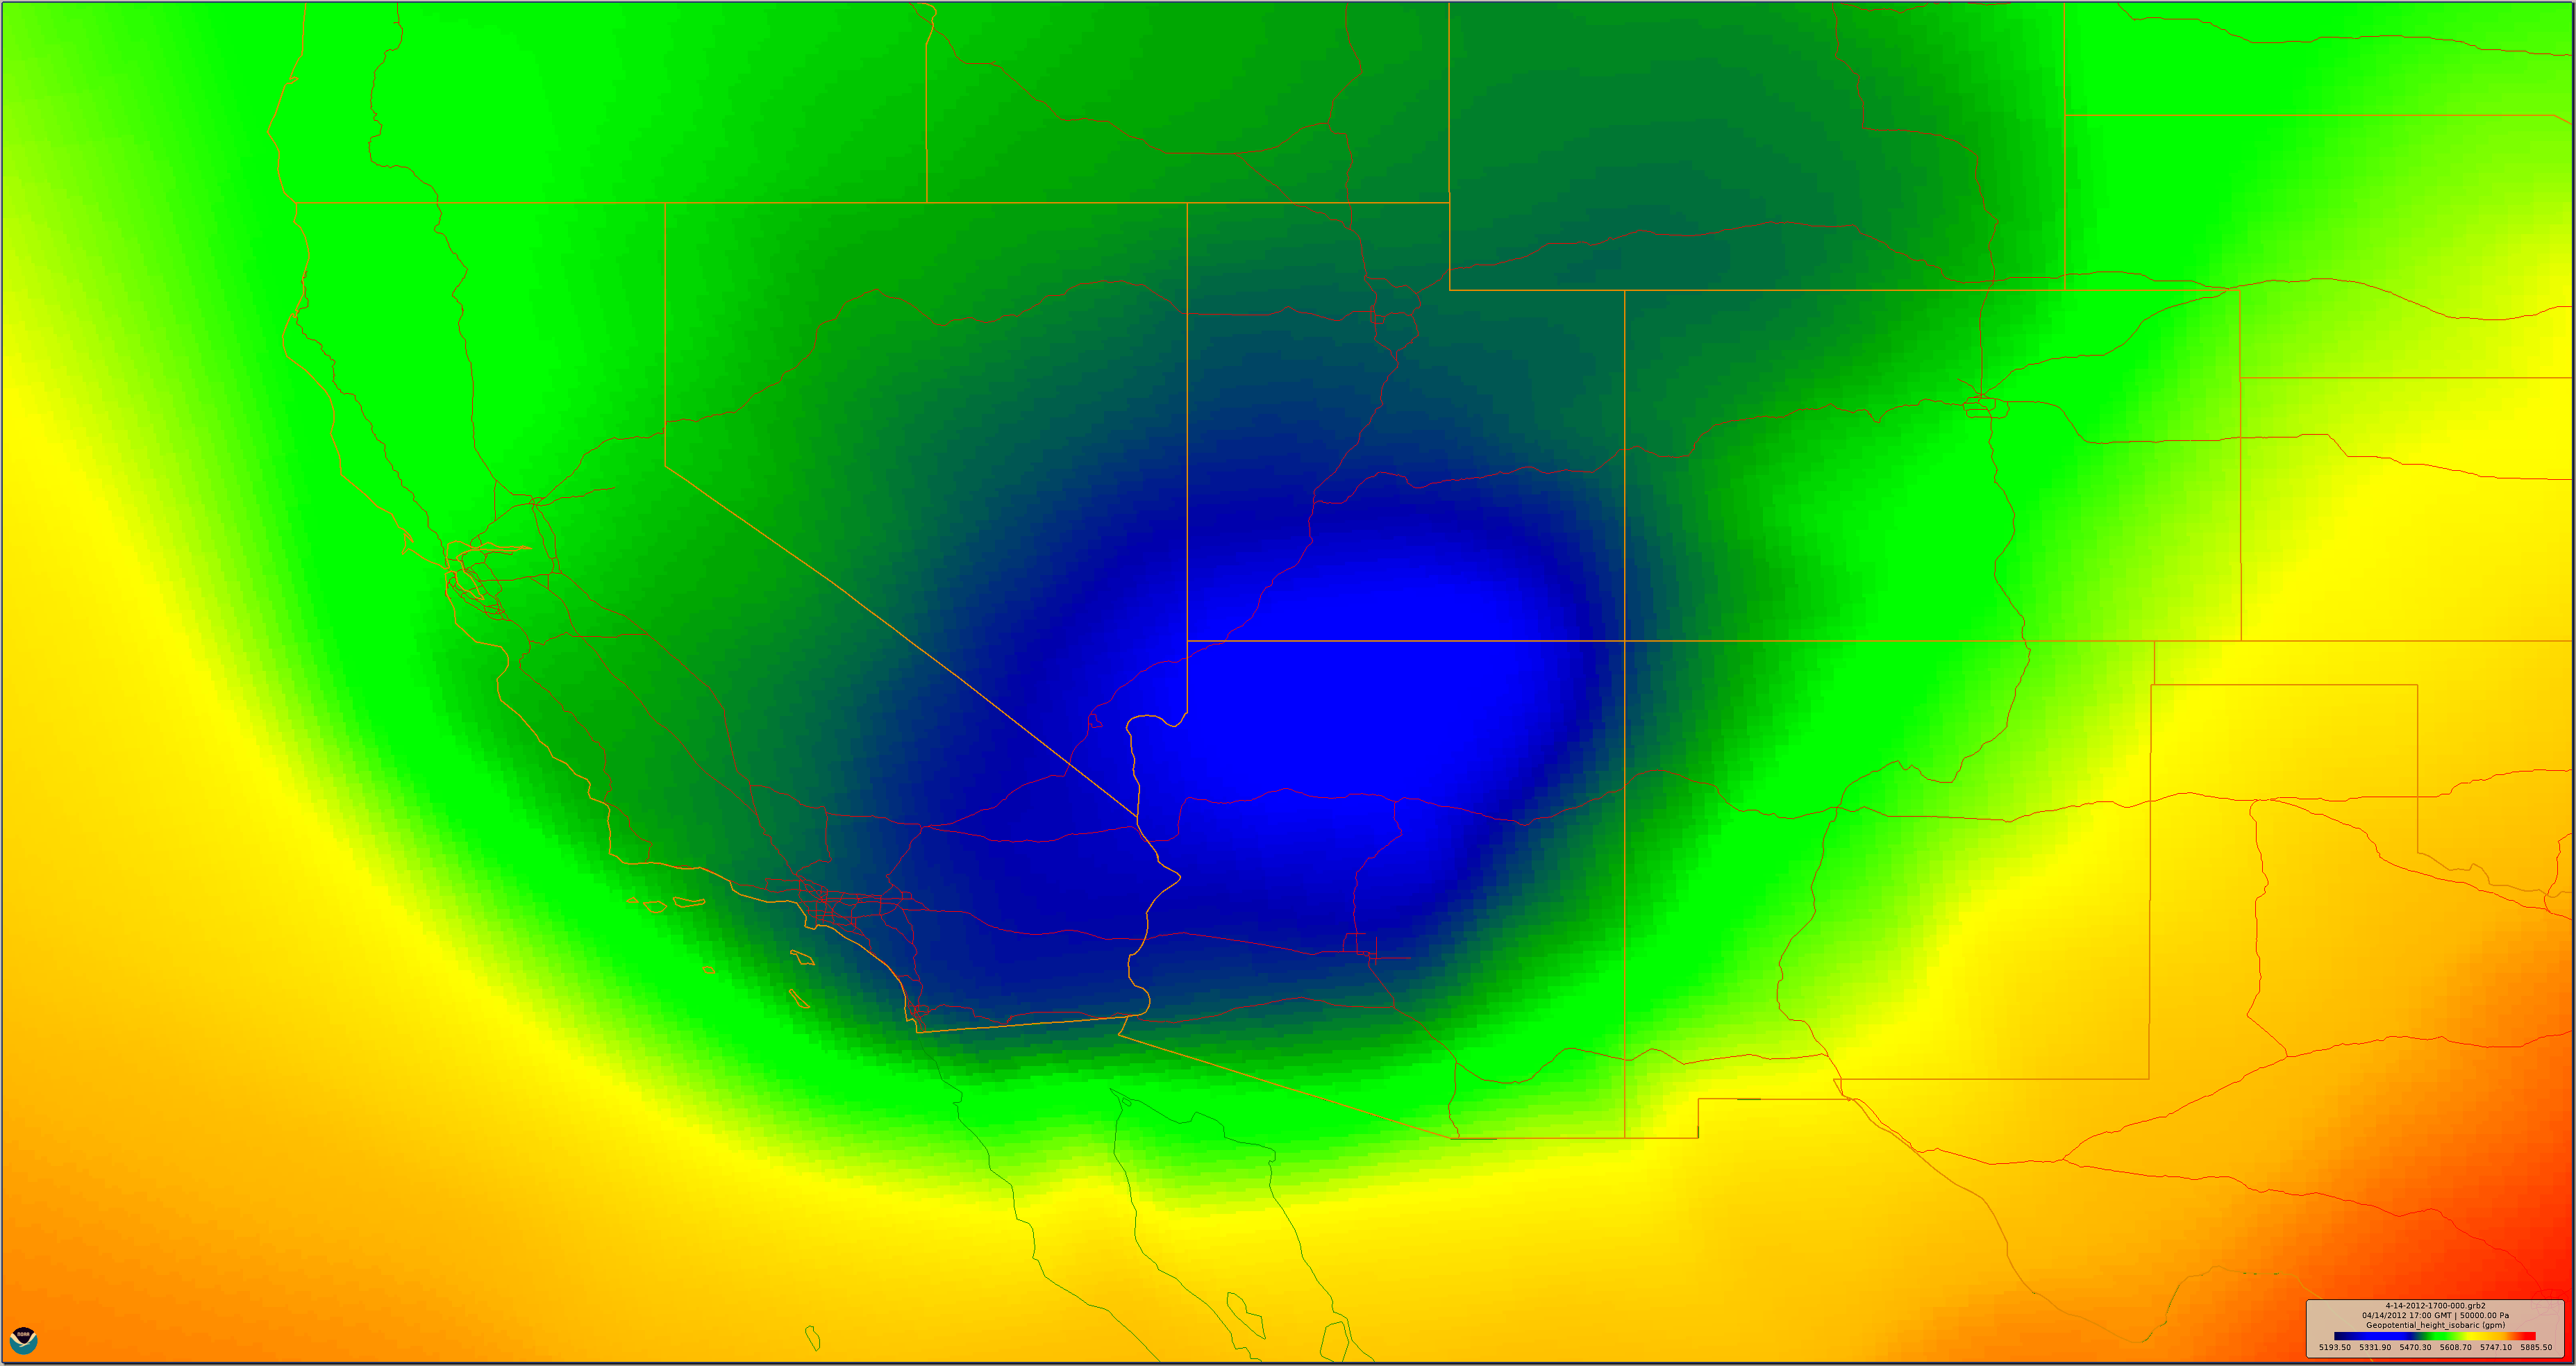
\includegraphics[width=\textwidth]{images/abqlow.png}
	\caption{Map of 500mB geopotential height during a major dust event on April 14, 2012, created using NOAA WCT viewer.}
\end{figure}

\subsection{Processing}
In order to get the data into a readable format for data mining and machine learning algorithms, the data must be recorded into a list of entries. Each entry is a vector of every parameter for a specific time and location. To achieve this format, the GRIB file for the desired time is opened, and for each gribmessage object in the file iterator, the value corresponding to the latitude and longitude is appended to a vector. That vector is then recorded to a CSV file for easier lookup in later processes. There is one CSV file for dust days, and another for non-dust days. In order to determine which dates are dusty, a list of dust events is gathered from the NOAA Storm Event Database. For any location, if a dust event occurred on a given date, the days before and after that date are removed from the dataset if they are not also dust dates. Doing so ensures a more obvious distinction between dust and non-dust dates.

If an algorithm is to use principal components instead of the raw data, a principal component analysis script will take the CSV files containing the weather data and write new CSV files containing the data in the form of the first $k$ principal components, where $k$ is specified in the script. After the CSV is written, a smaller fraction of the list of events is cut and pasted into a new CSV file, such that the larger file acts as the proper training data and the smaller is a set of data to test the model after training.
\pagebreak
\begin{figure}[H]
	\label{fig:pca}
	\subfigure[]{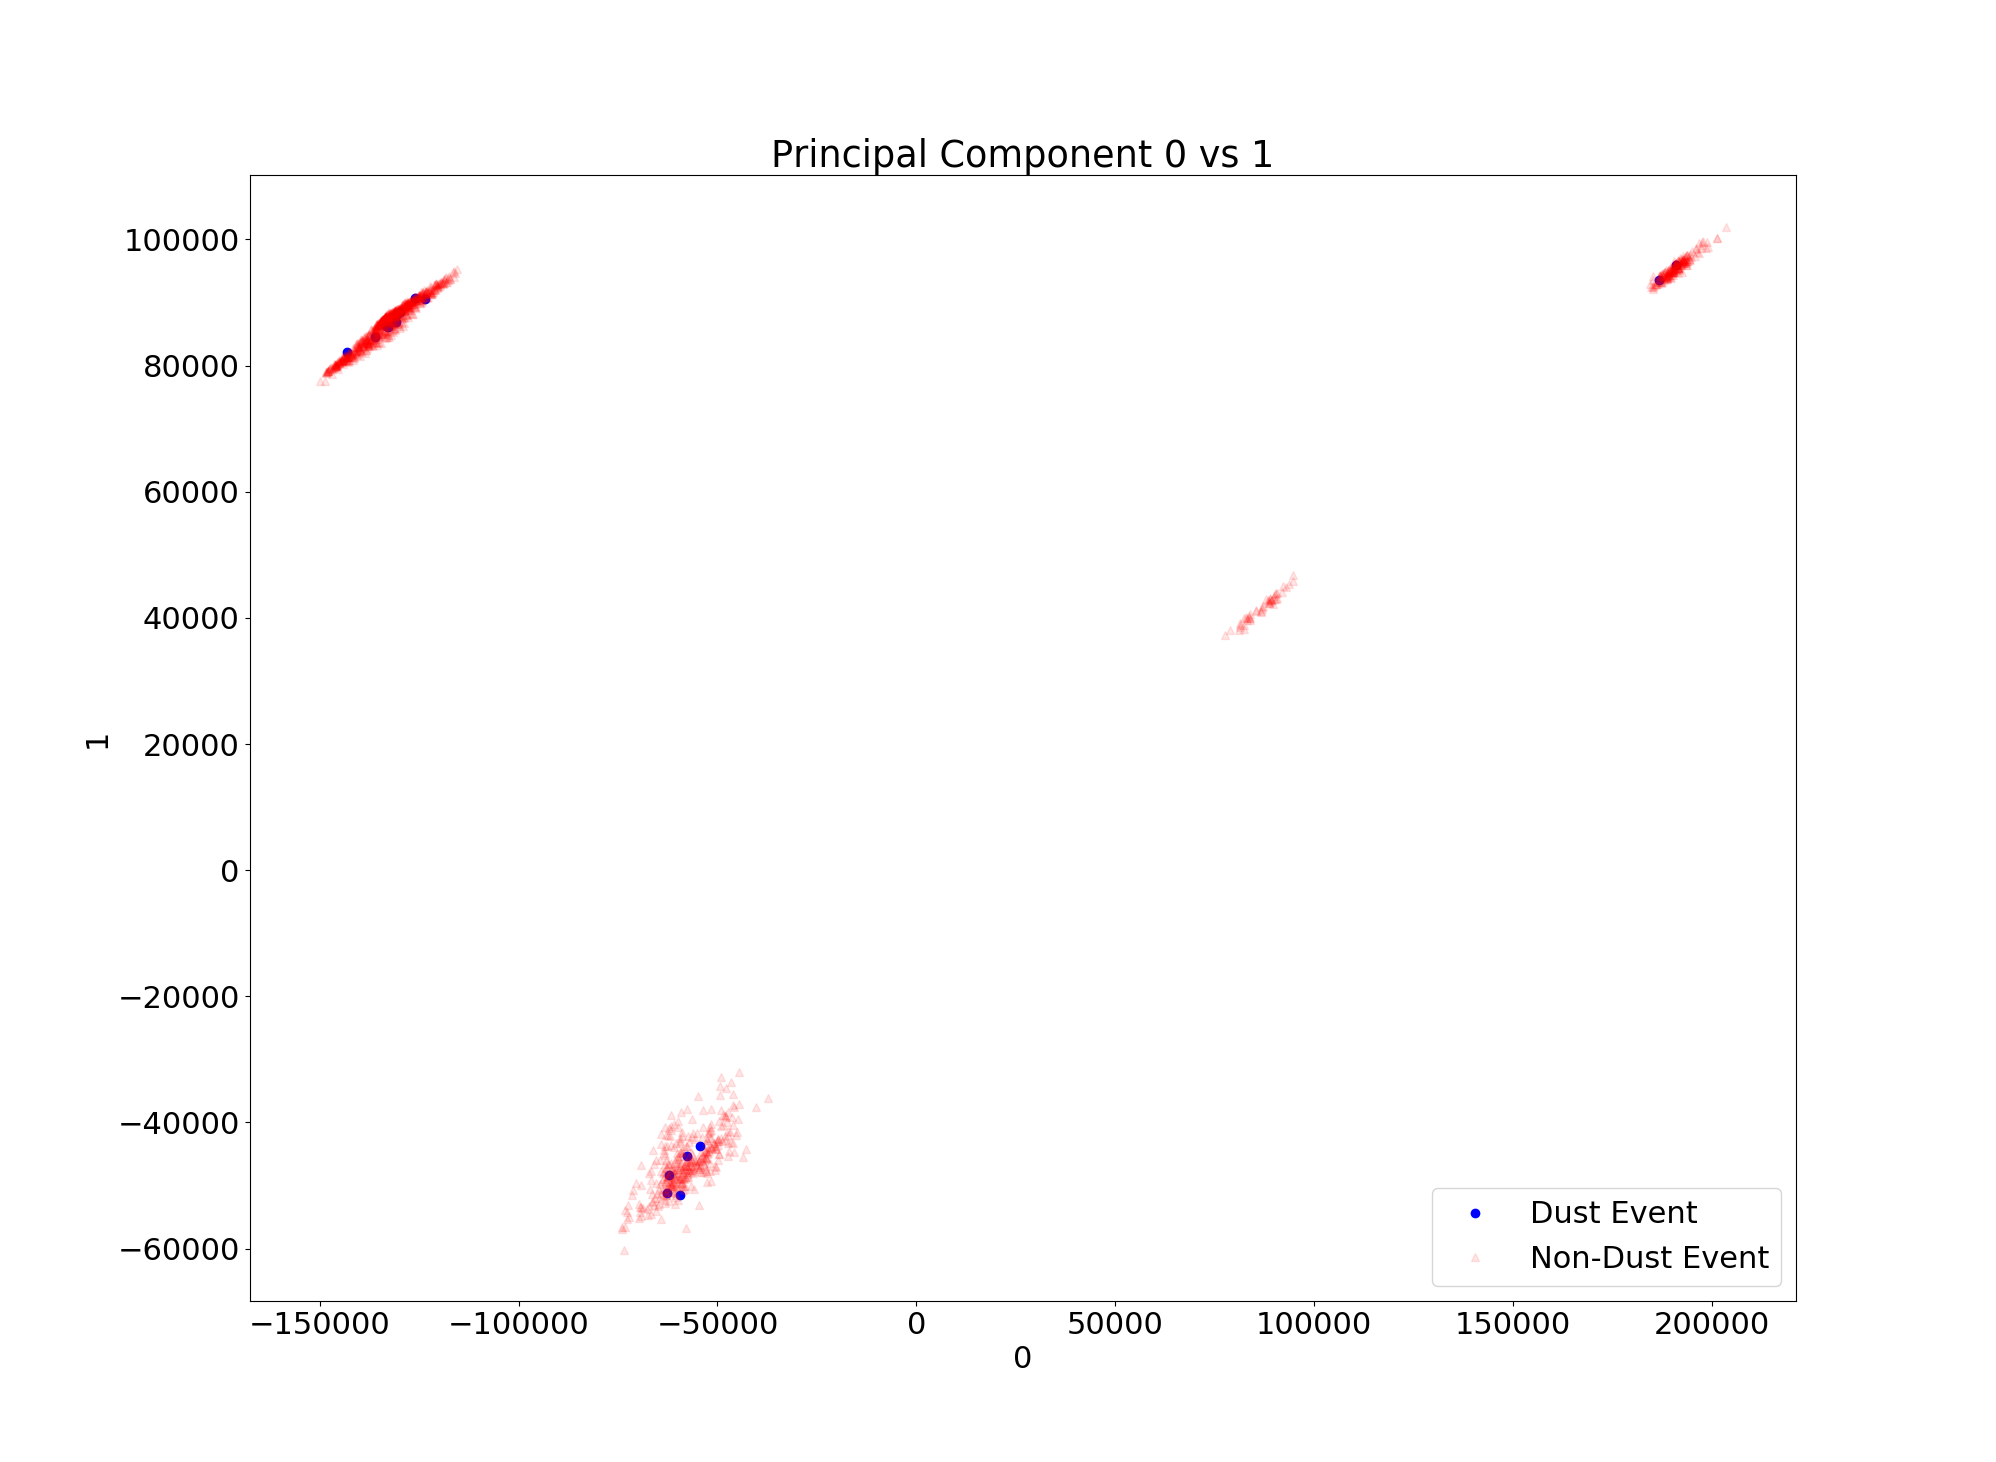
\includegraphics[width=0.9\textwidth]{images/0vs1.png}
		}
	\subfigure[]{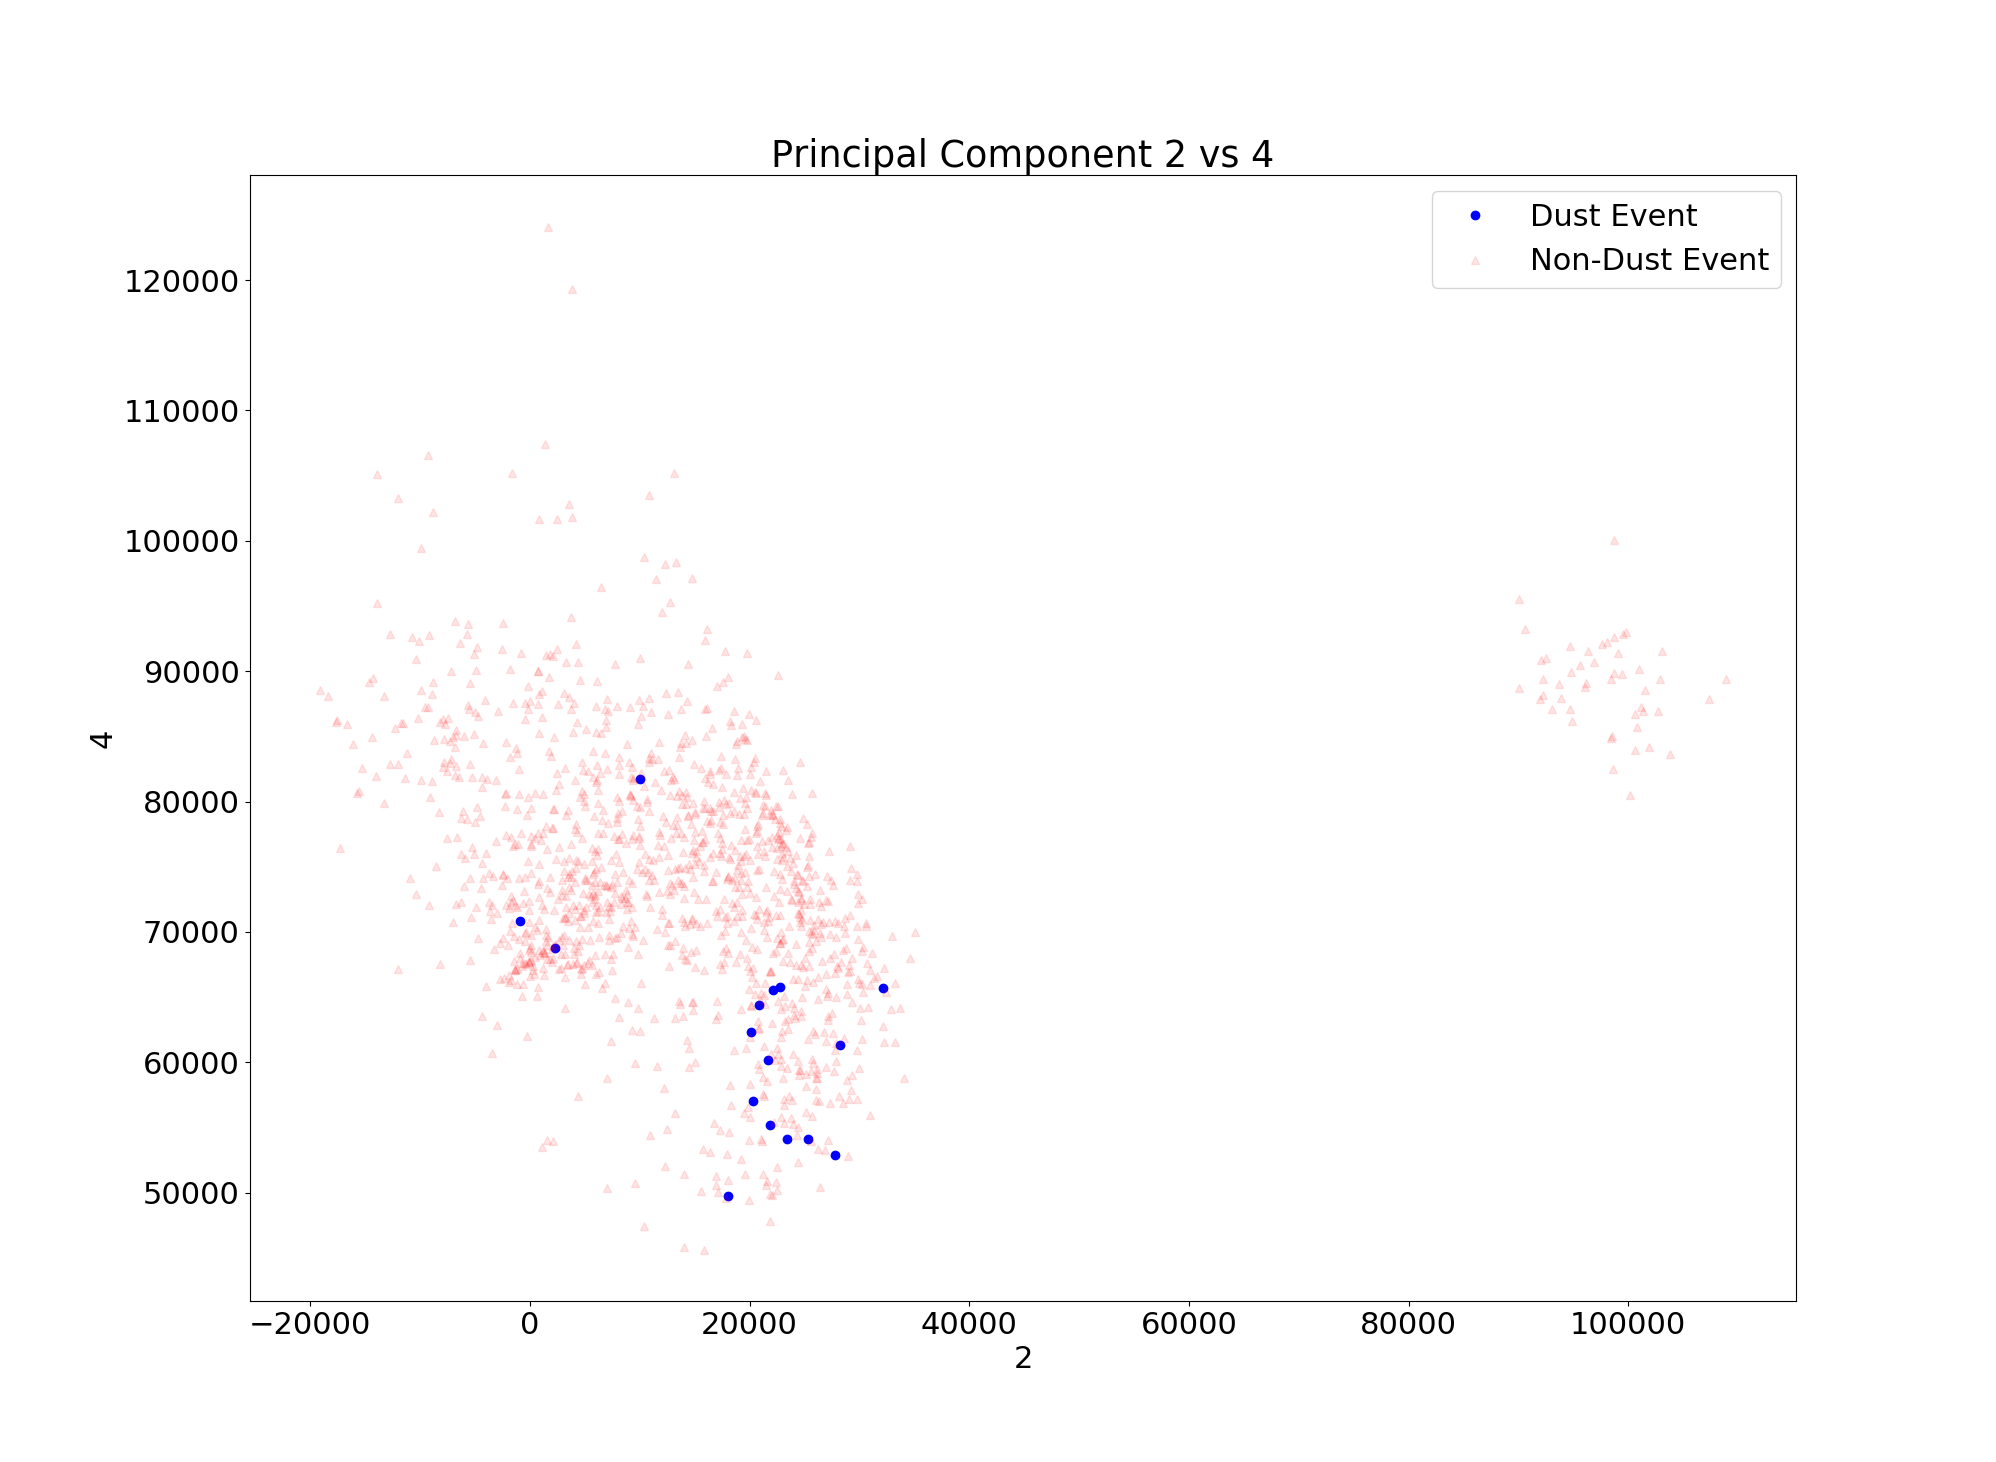
\includegraphics[width=0.9\textwidth]{images/2vs4.png}}
	\caption{Two scatter plots for principal components, one with no clear distinction between dust and nondust events (a), and one with some visible distinction (b).}
\end{figure}
\pagebreak


The plots in figure ~\ref{fig:pca} are taken from a PCA of data from the greater Phoenix area from 2008 to 2012. In this example, five components are taken. These plots are useful for determining whether there is a distinct separation in the data before using it to train a neural network and make predictions. 

For a preliminary predictive model, data will be taken from the dates of April 13, 2007 to April 30, 2012. This time range was selected because it is the largest set of consistent file format and number of parameters in the NOMADS RAP/RUC archive. 

\subsection{Modeling}
To finally create a predictive model for dust events, various types of neural networks are implemented. The number of inputs can either be the raw weather data or the principal components. The output is a single node, as this problem requires a binary classification of dust or non-dust events. The number of hidden layers and nodes can vary according to which input data is used. The first model is a simple feedforward neural network, using the raw data as input. Next is another feedforward network but with prinicpal components as the input. Recurrent neural network allow for a more context-sensitive model. The recurrent neural network models follow the long short-term memory (LSTM) architecture, which allows for previous information fed to the network to be remembered or forgotten over a specific period of time \cite{rnn}.

Each neural network model is implemented using the TensorFlow Python library. TensorFlow creates a graph of the computation performed and automates backpropagation for optimization algorithms. Each model created for this project uses TensorFlow's built-in gradient descent optimzer \cite{tfdoc}.

\subsection{Feedforward Neural Network}
The first neural network used for a predictive model is a simple feedforward net. The nodes in this neural network use a $tanh$ activation function, because the data does not follow a normal distribution and the sigmoid does not provide a steep enough gradient for optimization. With 10 principal components as inputs, networks of varying hidden layers of 25 nodes are tested to determine which provides the most accuracy. Because the dataset provided is imbalanced, the loss function is given weights such that a greater loss is calculated from a false negative than from a false positive.
\subsection{Recurrent Neural Network with LSTM}
The second type of neural network used as a predictive model is a recurrent neural network with a basic LSTM structure.
\section{Results}
\subsection{Feedforward Neural Netowrk}
The feedforward neural network provides preliminary results for possible predictive dust event models using neural networks. 
\subsection{Recurrent Neural Network with LSTM}
With a resolution of 24 hours, the recurrent neural network will achieve 89\% accuracy with the existing dataset. When observing the model's guessing pattern, it is found that this level of accuracy is not meaningful as even with the weighted loss function, the RNN guesses each event as non-dust. In order to create a model with more meaningful results, a dataset with a resolution of 24 hours would be more suitable. The training data used for this model does not have every successive event in the same location, so the LSTM cell makes a prediction using cell and hidden state information from a location possibly hundreds of kilometers away. In order to make a more useful LSTM model, a dataset with a resolution of 1 hour instead of 24 and beginning and end times of every dust event would allow for training based on 24-hour sequences for each recorded date instead of reading the entire list of events as a single sequence.

\begin{thebibliography}{4}
		\bibitem{unep}
			UNEP GEAS. "Forecasting and early warning of dust storms." UNEP. Feb. 2013. Web. May 24 2017. 
			\url{https://na.unep.net/geas/archive/pdfs/GEAS_Feb2013_DustStorm.pdf} 
		\bibitem{phairs}
			Benedict, Karl et. al. "Final Benchark Report." \textit{Public Health Applications in Remote Sensing}. Sep. 2008. Web. May 24 2017. \url{http://phairs.unm.edu/publ/Final%20Benchmark%20v14b%209-30-08.pdf}
		\bibitem{500mb} Armenta, Rebecca B. "Geopotential height patterns at 500mb associated with dust storms in the United States/Mexico border region during January-May of 2011-2014." May 2016 New Mexico State University.  Access May 31 2017.
		\bibitem{tan}
			Tan, P. Steinbach, M. Kumar, V. \textit{Introduction to Data Mining}. 2006 Pearson. Access May 23 2016. 
		\bibitem{wget} "GNU Wget 1.18 Manual." GNU Project. Web. Jun. 27 2017. \url{https://www.gnu.org/software/wget/manual/wget.html}
		\bibitem{rap}"Rapid Refresh (RAP)." National Centers for Envrionmental Information. NOAA. Web. Jun. 27. 2017. \url{https://www.ncdc.noaa.gov/data-access/model-data/model-datasets/rapid-refresh-rap}

		\bibitem{pgdoc} "pygrib documentation." Github. Dec. 29 2014. Web. Jun. 14 2017. \url{http://jswhit.github.io/pygrib/docs/}
		\bibitem{rnn} Zaremba, W. Sutskever, I. Vinyals, O. "Recurrent Neural Network Regularization." arXiv. Feb. 19 2015. Web. Jul. 5 2017. \url{https://arxiv.org/pdf/1409.2329.pdf}
		\bibitem{tfdoc} "Getting Started with TensorFlow." TensorFlow. Web. Jul. 5 2017. \url{https://www.tensorflow.org/get_started/get_started}


\end{thebibliography}

\end{document}
